
Gospodarka składa się z zon i zasobów oraz grup politycznych. Naturalnie w przyrodzie występują tylko zasoby surowcowe (S) i energetyczne (E).

Przestrzeń gospodarki jest podzielona na zony (Z). Do zon przypisane są zasoby surowcowe i energetyczne.


\begin{figure}[h!]
    \centering
    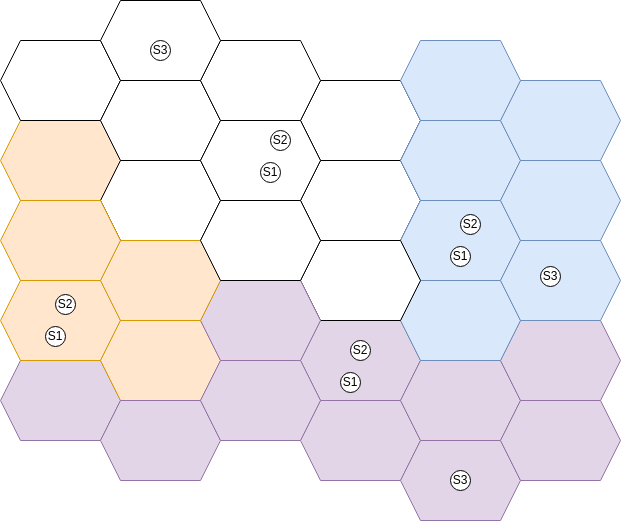
\includegraphics[width=0.8\textwidth]{img/zony.drawio.png}
    \caption{Przykład podziału przestrzeni na zony jako siatka hexagonalna, z przypisanymi zasobami}
    \label{fig:zony}
    \end{figure}

Grupa polityczna zajmuje określone zony, przez co i zasoby.

Z zasobów naturalnych można produkować zasoby wyższego poziomu, przemysłowe oraz high-tech. 

Celem grupy politycznej jest zdobycie jak największej ilości zasobów, aby produkować zasoby wyższego poziomu i zdobywać przewagę nad innymi grupami politycznymi.

Grupa polityczna ma dwa rodzaje interakcji z innymi grupami politycznymi:
\begin{itemize}
    \item \textbf{Interakcje pokojowe} - grupy polityczne mogą tworzyć sojusze, wymieniać się zasobami, aby produkować zasoby wyższego poziomu.
    \item \textbf{Interakcje militarne} - grupy polityczne mogą atakować inne grupy polityczne, aby zdobyć ich zony i zasoby.
\end{itemize}





\begin{figure}[h!]
\centering
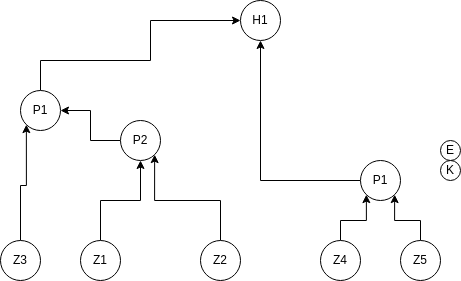
\includegraphics[width=0.8\textwidth]{img/zasoby.drawio.png}
\caption{Schemat zasobów}
\label{fig:zasoby}
\end{figure}



\section*{Przestrzeń gospodarki}

Gospodarka to graf złożony z węzłów i krawędzi. Węzły to zony, a krawędzie to połączenia między zonami.
Graficznie przestrzeń tworzy hexagonalną siatkę, w której każda zona ma 6 sąsiadów.

Hexagonalna siatka może być opisana za pomocą współrzędnych osiowych (axial coordinates), które definiują pozycję każdej zony w przestrzeni. Współrzędne te są oznaczane jako \( (q, r) \), gdzie \( q \) i \( r \) to liczby całkowite.

Odległość między dwoma zonami w hexagonalnej siatce można obliczyć za pomocą wzoru:
\[
d = \frac{|q_1 - q_2| + |q_1 + r_1 - q_2 - r_2| + |r_1 - r_2|}{2}
\]
gdzie \( (q_1, r_1) \) i \( (q_2, r_2) \) to współrzędne dwóch zon.

Hexagonalna siatka może być również przedstawiona graficznie, gdzie każda zona ma sześciu sąsiadów, a ich współrzędne są przesunięte o stałą wartość w zależności od kierunku.


\section*{Inne możliwości}

\begin{itemize}
    \item Niektóre zasoby na początku rozgrywki nie są przypisane do żadnej grupy politycznej. Grupa polityczna może je zdobyć, zajmując odpowiednią zonę.
\end{itemize}